\documentclass[tikz,border=8pt]{standalone}

\usepackage[T1]{fontenc}
\usepackage[utf8]{inputenc}
\usepackage{tikz}
\usetikzlibrary{positioning,arrows.meta}
\usetikzlibrary{calc}

\tikzset{
    >=Stealth,
    module/.style={
        rectangle,
        rounded corners,
        draw,
        align=center,
        minimum width=4.0cm,
        minimum height=1.25cm
    },
    data/.style={
        rectangle,
        draw,
        align=center,
        minimum width=4.0cm,
        minimum height=1.0cm
    }
}

\begin{document}

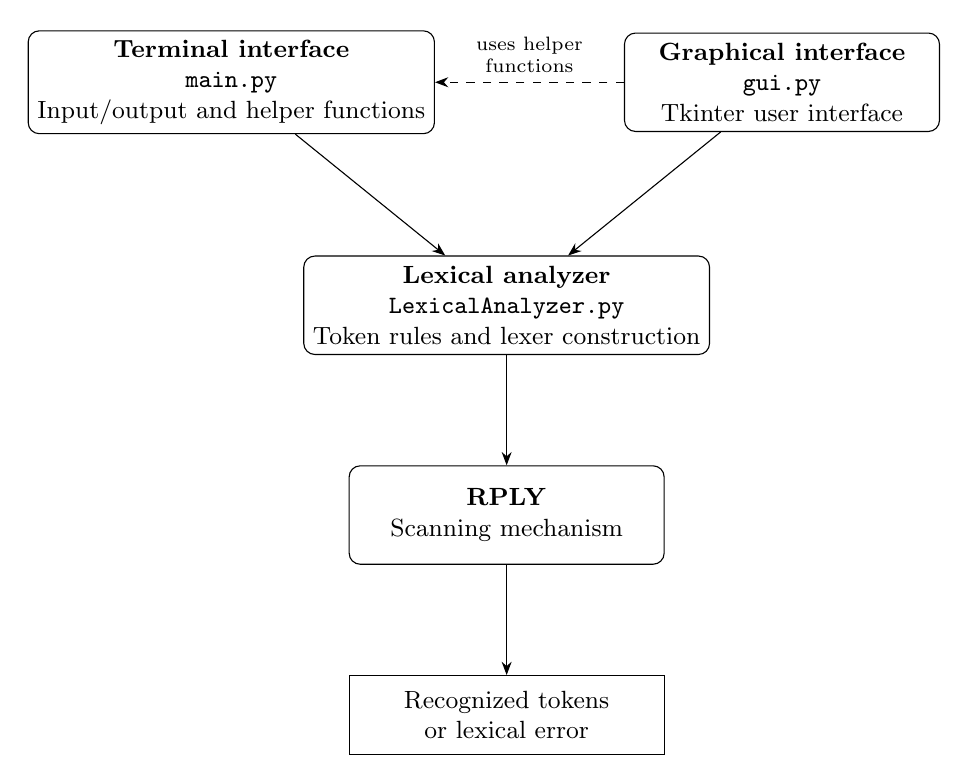
\begin{tikzpicture}[
    node distance=14mm and 24mm,
    font=\small,
    ->
]

% Interfaces
\node[module] (main)
{
\textbf{Terminal interface}\\
\texttt{main.py}\\
Input/output and helper functions
};

\node[module, right=of main] (gui)
{
\textbf{Graphical interface}\\
\texttt{gui.py}\\
Tkinter user interface
};

% Shared lexer
\node[module, below=22mm of $(main)!0.5!(gui)$] (lexer)
{
\textbf{Lexical analyzer}\\
\texttt{LexicalAnalyzer.py}\\
Token rules and lexer construction
};

% RPLY
\node[module, below=of lexer] (rply)
{
\textbf{RPLY}\\
Scanning mechanism
};

% Result
\node[data, below=of rply] (result)
{
Recognized tokens\\
or lexical error
};


% Both interfaces use the lexer
\draw (main) -- (lexer);
\draw (gui) -- (lexer);

% Lexer uses RPLY
\draw (lexer) -- (rply);

% Output of scanning
\draw (rply) -- (result);

% GUI also uses helper functions from main
\draw[dashed, ->]
    (gui.west)
    -- node[midway, above, font=\scriptsize, align=center]
    {uses helper\\functions}
    (main.east);

\end{tikzpicture}

\end{document}